\section{Probabilistic Inference}\label{cha:probReasoning} 

We have investigated means to store the knowledge about a system and now turn to the retrieval of information, a process called inference.


\begin{remark}[Interpretation of Contractions in Probabilistic Reasoning]
	Contraction compute marginal distributions, where the marginal variables are on the open legs of the contraction.
\end{remark}

% 
Contraction of the relational encoding of a function with a Markov Network gives the statistics over the values of the functions.
When contracting the function directly, we get the expectation.

% Message passing
%Another approximation comes from an approximation of the contractions itself. 
One can increase the efficiency of inference algorithms by using approximative contractions.
Here, message passing schemes can be applied as to be introduced in Chapter~\ref{cha:localContractions}.

\subsection{Queries}

Let us now formalize queries by contractions.

\subsubsection{Querying by functions}

We can formalize queries by retrieving expectations of functions given a distribution specified by probability tensors. 

\begin{definition}\label{def:queries}
	The query of a probability distribution $\probof{\shortcatvariables}$ by a tensor 
		\[ \exfunction : \facstates \rightarrow \rr \]
	is the vector $\probof{\catvariableof{\exfunction}} \in \rr^{\cardof{\imageof{\exfunction}}}$ defined as the contraction
	\begin{align*}
		\probof{\catvariableof{\exfunction}} = \contractionof{\probof{\shortcatvariables},\rencodingofat{\exfunction}{\shortcatvariables,\catvariableof{\exfunction}}}{\catvariableof{\exfunction}} \, . 
	\end{align*}
	Given another tensor $\secexfunction: \facstates \rightarrow \rr $ the conditional query of the probability distribution $\probof{\shortcatvariables}$ by the tensor $\exfunction$ conditioned on the tensor $\secexfunction$ is the matrix $\condprobof{\exfunction}{\secexfunction}\in\rr^{\cardof{\imageof{\exfunction}}}\otimes \rr^{\cardof{\imageof{\secexfunction}}}$ defined as the normation
	\begin{align*}
		\condprobof{\catvariableof{\exfunction}}{\catvariableof{\secexfunction}} 
		= \normationofwrt{\{
		\probof{\shortcatvariables},\rencodingofat{\exfunction}{\shortcatvariables,\catvariableof{\exfunction}},\rencodingofat{\secexfunction}{\shortcatvariables,\catvariableof{\secexfunction}}
		\}}{
		\catvariableof{\exfunction}}{\catvariableof{\secexfunction}
		} \, . 
	\end{align*}
\end{definition}

%% Conditional Probabilities and conditional queries
Conditional probabilities are queries, where the tensors $\exfunction$ and $\secexfunction$ are identity mappings in the respective variable state spaces.
Conversely, we can understand the conditional query $\condprobof{\exfunction}{\secexfunction}$ as the conditional probability of $\exfunction$ conditioned on $\secexfunction$, of the underlying Markov Network with cores $\{\probtensor, \rencodingof{\exfunction}, \rencodingof{\secexfunction} \}$ and variables $\catvariableof{\exfunction},\catvariableof{\secexfunction}$ besides the variables distributed by $\probtensor$.

%% Expectations as event queries -> Consistency with $\probof{X=i}$?
We further denote event queries by
	\[  \expectationof{\exfunction=z} = \sbcontractionof{\probtensor,\rencodingof{\exfunction},\onehotmapof{z}}{\varnothing} \]
where by $\onehotmapof{z}$ be denote the one hot encoding of the state $z$ with respect to some enumeration.
Let us note that they are further contraction of the queries in Definition~\ref{def:queries} since by Theorem~\ref{the:splittingContractions}
\begin{align*}
	 \expectationof{\exfunction=z} 
	& =  \sbcontractionof{ \sbcontractionof{\probtensor,\rencodingof{\exfunction}}{\catvariableof{\exfunction}} ,\onehotmapof{z}}{\varnothing} \\
	& =  \sbcontractionof{ \probof{\exfunction} ,\onehotmapof{z}}{\varnothing} \, . 
\end{align*}

%% OLD: Defining queries by 
%\begin{definition}
%	The expectation of functions $\exfunction$ given a probability tensor is the contraction
%		\[ \expectationofwrt{\exfunction(\catvariables)}{\catvariables\sim\probtensor} = 
%			\contractionof{\{\probtensor,\rencodingof{\exfunction}\}}{\{\exfunctiontargetvariables \}} \, . 
%		\]
%\end{definition}
%This is the canonical definition of expectations, since summing function values weighted by the probability of the argument.
%When we have an unnormalized probability distribution $\phi$ the expectation is the quotient
%\begin{align*}
%	\expectationofwrt{\exfunction(\catvariables)}{\catvariables\sim\phi}  = \frac{
%		\contractionof{\{\phi,\ftensorof{\exfunction}\}}{\{\exfunctiontargetvariables \}} 
%	}{
%		\contractionof{\{\phi\}}{\varnothing} 
%	} \, . 
%\end{align*}

%\subsubsection{Conditional Probability Queries}
%
%Typical queries are the computation of an a posteriori distribution given evidence.
%This is just the contraction.
%
%%% As expectation
%The query consists of the one-hot encoding of the evidence and Ids elsewhere.
%The result is then interpreted as another probability distribution, defined as a Markov network and the possible need to normalize with the partition function.
%
%Given evidence, condition the probability tensor on that evidence.




\subsubsection{MAP Queries}

Find the maximal variable of the (conditioned) probability tensor.

Given a probability tensor the search for its maximal coordinate is 
\begin{align}
	\argmax_{\catindices} \probof{\indexedcatvariables} \, .
\end{align}

Often, the generation of a full (conditioned) probability tensor can be infeasible, if too many variables are queries.
Having a tensor network decomposition of the probability tensor avoids this generation.

Along this we reformulate the maximal coordinate problem as
\begin{align}
	\argmax_{\catindices} \probof{\indexedcatvariables} 
	= \argmax_{\catindices} \contractionof{\{\probtensor, \onehotmapof{\catindices}\}}{\varnothing}  \, .
\end{align}

We understand it as a Tensor Network approximation problem, where the approximating tensor are the one-hot encodings of states.


\red{MAP queries are approximated by sampling from annealed distributions.}

\begin{remark}\label{rem:simulatedAnnealing}
% Simulated annealing
	\red{Here by the naive exponential family}
	Simulated annealing manipulates the probability used to sample $\atomlegindexof{\atomenumerator}$ in terms of an inverse temperature parameter $\invtemp$, by
		\[ \probtensor \rightarrow \frac{\expof{\invtemp\cdot\lnof{\probtensor}}}{\contractionof{\expof{\invtemp\cdot\lnof{\probtensor}}}{\varnothing} } \, . \]
	When the temperature is larger than $1$, the probability of states with low probability increases while the probability of states with large probability decreases and for low temperatures the opposite.
	Simulated annealing, that is the decrease of the temperature to $0$ during Gibbs sampling biases the algorithm towards states with large probability.
%	Tuning this parameter can improve the convergence of Gibbs Sampling.

	% On exponential families
	For any exponential family the transformation 
		\[ \energytensor \rightarrow \invtemp \cdot \energytensor  \]
	can be performed by rescaling the canonical parameters as
		\[ \canparam \rightarrow \invtemp \cdot \canparam \, . \]
\end{remark}





\subsection{Sampling}

Let us here investigate how to draw samples from distributions $\probtensor$.

%Need to generate the full conditional probability distribution by contraction and then sample from it.
Since there are $\prod_{\node\in\nodes}\catdimof{\node}$ coordinates stored in $\probtensor$, naive methods are often infeasible.
One can instead exploit a representation of $\probtensor$ by a Markov network or the energy term in an exponential family for efficient algorithms.
%\begin{itemize}
%	\item Empirical Distribution: Use the basis CP Decomposition and sample by choice of a random slice
%	\item Bayesian Network: Starting from the leaves sample 
%\end{itemize}

\subsubsection{Exact Methods}

Forward Sampling (see Algorithm~\ref{alg:ForwardSampling}) uses a chain decomposition (see Theorem~\ref{the:chainRule}) of a probability distribution to iteratively sample the variables.

\begin{algorithm}[hbt!]
\caption{Forward Sampling}\label{alg:ForwardSampling}
\begin{algorithmic}
\For{$\atomenumeratorin$}
	\State Draw $\atomlegindexof{\atomenumerator}\in[\catdimof{\atomenumerator}]$ from conditional distribution 
		\[ \condprobof{\catvariableof{\atomenumerator}}{\{\catvariableof{\secatomenumerator} = \atomlegindexof{\secatomenumerator} \, : \, \secatomenumerator < \atomenumerator \}} \]
%		\onehotmapof{\atomlegindexof{\secatomenumerator}} \, : \secatomenumerator < \atomenumerator\}}  \] 
\EndFor
\end{algorithmic}
\end{algorithm}





%% Comment on rejection Sampling - required?
% Conditioned Sampling
When sampling from conditional probability distributions, one can sample from the conditioned distribution instead.
However, the conditioning changes the structure of the distribution, and conditioned Bayesian Networks are not Bayesian Networks on the same graph.
One ways around is rejection sampling, where one samples from the unconditioned distribution and rejects samples not satisfying the event conditioned on.
When the event conditioned on is of small probability, methods like rejection sampling will come with large runtimes.

\subsubsection{Approximate Methods}

% Problem of many variables
When there are many variables to be sample, the computation of the conditional probability to all variables can be infeasible.
One way to overcome this is Gibbs Sampling: Iteratively resemble single variables given the rest as evidence.

%\subsubsection{Gibbs Sampling}

% Still old: Sample from Marginal
Sample each variable independent from the marginal distribution.
Then, alternate through the variables and sample each variable from the conditional distribution taking the others as evidence.

\begin{algorithm}[hbt!]
\caption{Gibbs Sampling}\label{alg:Gibbs}
\begin{algorithmic}
\For{$\atomenumeratorin$}
	\State Draw State for atom $\atomenumerator$ from initialization distributions. % In implementation: Initialize with ones and draw -> Avoids zero probability state
\EndFor
\While{Stopping criterion is not met}
\For{$\atomenumeratorin$}
	\State Draw $\atomlegindexof{\atomenumerator}\in[\catdimof{\atomenumerator}]$ from 
		\[ \condprobof{\catvariableof{\atomenumerator}}{\{\catvariableof{\secatomenumerator}=\atomlegindexof{\secatomenumerator} \, : \secatomenumerator \neq \atomenumerator\}} \]
		%= 
		%\frac{
		%\contractionof{\{\probtensor\} \cup \{\onehotmapof{\atomlegindexof{\secatomenumerator}} \, : \secatomenumerator \neq \atomenumerator \}}{\catvariableof{\atomenumerator}}
		%}{
		%\contractionof{\{\probtensor\} \cup \{\onehotmapof{\atomlegindexof{\secatomenumerator}} \, : \secatomenumerator \neq \atomenumerator \}}{\varnothing}
		%} \]
\EndFor
\EndWhile
\end{algorithmic}
\end{algorithm}


% Energy
Let us now interpret a probability tensor at hand as a member of an exponential family (see Section~\ref{sec:exponentialFamilies}), which is always possible when taking the naive exponential family.
Gibbs sampling can be implemented based on the energy tensor $\energytensor$ of the probability tensor, using
	\[ \condprobof{\catvariableof{\atomenumerator}}{\{\catvariableof{\secatomenumerator}=\atomlegindexof{\secatomenumerator} \, : \secatomenumerator \neq \atomenumerator\}} = \normationofwrt{\expof{\contractionof{\{\energytensor\}\cup\{\onehotmapof{\atomlegindexof{\secatomenumerator}} \, : \secatomenumerator \neq \atomenumerator \}}{\catvariableof{\atomenumerator}}}}{\catvariableof{\atomenumerator}}{\varnothing}  \, .\]
Thus, it suffices to build the selection encoding of the statistics, and we can avoid the usage of the relational encoding.
\red{This is in contrast with forward sampling, where we need to sum over many coordinates of the exponentiated energy tensor, which amounts to the representation of the probability distribution as a tensor network using relational encodings.}
%where the operation with energy tensors and selection encodings is not efficient.}










\subsection{Maximum Likelihood Estimation} % Stuff from Parameter Estimation - Problem that Part I is called inference?

Let us now turn to inductive reasoning tasks, where a probabilistic model is trained on given data.

\subsubsection{Likelihood and Cross Entropy}

Given a datapoint $\datapointof{\dataindex}$ consisting of the images of the data selecting map $\datamap$ (see Definition~\ref{def:dataMap}), the likelihood given a Markov Logic Network is denoted as
	\[ \probof{\shortcatvariables = \datamapof{\dataindex}} \, . \]
	
% Independent assumption
When all $\datamapof{\dataindex}$ are drawn independently from $\mlnprobat{\shortcatvariablelist}$, we can factorize into
	\[ \probof{\data}  = \prod_{\dataindexin} \probof{\shortcatvariables=\datamapof{\dataindex}} \, . \]

% Logarithm
It is convenient to apply a logarithm on the objective, which does not influence the optimum.
This is especially useful, when investigating the convergence of the objective for $\datanum\rightarrow\infty$ (see Chapter~\ref{cha:mlnConcentration}).
We define the loss of a distribution $\probtensor$ as
\begin{align}\label{eq:defLikelihoodLossPL}
	\lossof{\probtensor} 
	= \frac{1}{\datanum} \lnof{\probof{\data}} 
\end{align}

\begin{lemma}
	The loss has the form 
	\begin{align}
		\lossof{\probtensor} = \contractionof{\{\empdistribution,\lnof{\probtensor}\}}{\varnothing}
	\end{align}
\end{lemma}
\begin{proof}
	We have
	\begin{align*}
		\lossof{\probtensor} 
		& = \frac{1}{\datanum} \lnof{\probof{\data}} 
		= \frac{1}{\datanum} \sum_{\datain} \lnof{\probof{\shortcatvariables =\datamap(\dataindex)}} 
		= \frac{1}{\datanum} \sum_{\datain} \contractionof{\{\lnof{\probtensor},\onehotmapof{\datamap(\dataindex)}\}}{\varnothing} \\ 
		& = \contractionof{\{\empdistribution,\lnof{\probtensor}\}}{\varnothing} \, .
	\end{align*}
\end{proof}

We thus state the Maximum Likelihood Problem in the form
\begin{align}\tag{$\mathrm{P}_{\lossof{}, \empdistribution}$}\label{prob:parameterMaxLikelihood}
	\argmin_{\probtensor\in\Gamma} \lossof{\probtensor} \, . % Naive Exponential Family perspective!
\end{align}



% M-Projection -> A projection since P^2 = P, i.e. P applied on the image is id
Most general, the Maximum Likelihood Problem is the M-Projection of a distribution $\gendistribution$ onto a set $\Gamma$ of probability tensors is
\begin{align}
	\argmax_{\probtensor\in\Gamma}  \centropyof{\gendistribution}{\probtensor} 
\end{align}
where the Maximum Likelihood Estimation is the special case $\gendistribution=\empdistribution$.




%% From Probability Representation
\subsubsection{Entropic Interpretation}

\begin{definition}[Shannon entropy]
	The information content or the Shannon entropy of a distribution is defined as
		\[ \sentropyof{\probtensor} := \expectationofwrt{-\lnof{\probof{\randomx}}}{\randomx\sim\probtensor} = - \sum_{\catindices} \probof{\indexedcatvariables} \cdot \lnof{\probof{\indexedcatvariables}} \, . \]
	We depict this in a tensor network diagram with an ellipsis denoting a coordinatewise transform (here the $\ln$) as:
	\begin{center}
		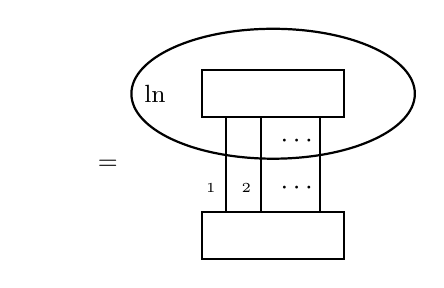
\begin{tikzpicture}[scale=0.3,thick] % , baseline = -3.5pt

\node[anchor=center] (text) at (-8,-5) {\small $\sentropyof{\probtensor}$};

\node[anchor=center] (text) at (-5,-5) {\small ${=}$};

\node[anchor=center] (text) at (-3,-2) {\small $\mathrm{ln}$};
\draw (2,-2) ellipse (6 and 2.75);

\draw (-1,-1) rectangle (5,-3);
\node[anchor=center] (text) at (2,-2) {\small $\probtensor$};
\draw (-1,-7) rectangle (5,-9);
\node[anchor=center] (text) at (2,-8) {\small $\probtensor$};
\draw (0,-5)--(0,-3); 
\draw (0,-5)--(0,-7) node[midway,left] {\tiny $\atomlegindexof{1}$}; 
\draw (1.5,-5)--(1.5,-3); 
\draw (1.5,-5)--(1.5,-7) node[midway,left] {\tiny $\atomlegindexof{2}$}; 
\node[anchor=center] (text) at (3,-4) {$\cdots$};
\draw (4,-5)--(4,-3);
\node[anchor=center] (text) at (3,-6) {$\cdots$};
\draw (4,-5)--(4,-7) node[midway,right] {\tiny $\atomlegindexof{\atomorder}$}; 

%\drawatomcore{3.5}{-8}{$\probtensor$}
%\drawatomindices{3.5}{-12}	
%\draw (5.5,-9)--(5.5,-7) node[midway,right] {\tiny $\atomlegindexof{\exformula}$};

\end{tikzpicture}
	\end{center}
\end{definition}

%We can use the Slicing theorem to ease the computation of the Shannon entropy.
%\red{Can be generalized to any Tensor being a sum of binary tensors. Thus topic better in binary tensor calculus?}

\begin{definition}[Cross entropy]\label{def:crossEntropy}
	The cross entropy between two distributions is defined as 
		\[ \centropyof{\probtensor}{\tilde{\probtensor}} 
		=  \expectationofwrt{-\lnof{\probof{\randomx}}}{\randomx\sim\probtensor} 
		= - \sum_{\catindices}  \probof{\indexedcatvariables} \cdot \lnof{\tilde{\probtensor}[\indexedcatvariables]}  \, . \]
	We depict this in a tensor network diagram with an ellipsis denoting a coordinatewise transform (here the $\ln$) as :
	\begin{center}
		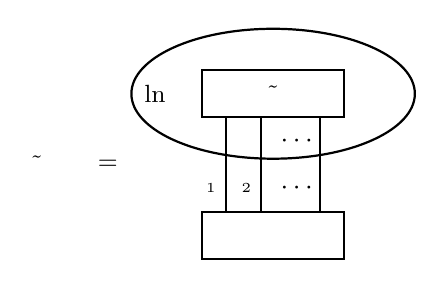
\begin{tikzpicture}[scale=0.3,thick] % , baseline = -3.5pt

\node[anchor=center] (text) at (-8,-5) {\small $\centropyof{\probtensor}{\tilde{\probtensor}}$};

\node[anchor=center] (text) at (-5,-5) {\small ${=}$};

\node[anchor=center] (text) at (-3,-2) {\small $\mathrm{ln}$};
\draw (2,-2) ellipse (6 and 2.75);

\draw (-1,-1) rectangle (5,-3);
\node[anchor=center] (text) at (2,-2) {\small $\tilde{\probtensor}$};
\draw (-1,-7) rectangle (5,-9);
\node[anchor=center] (text) at (2,-8) {\small $\probtensor$};
\draw (0,-5)--(0,-3); 
\draw (0,-5)--(0,-7) node[midway,left] {\tiny $\atomlegindexof{1}$}; 
\draw (1.5,-5)--(1.5,-3); 
\draw (1.5,-5)--(1.5,-7) node[midway,left] {\tiny $\atomlegindexof{2}$}; 
\node[anchor=center] (text) at (3,-4) {$\cdots$};
\draw (4,-5)--(4,-3);
\node[anchor=center] (text) at (3,-6) {$\cdots$};
\draw (4,-5)--(4,-7) node[midway,right] {\tiny $\atomlegindexof{\atomorder}$}; 

%\drawatomcore{3.5}{-8}{$\probtensor$}
%\drawatomindices{3.5}{-12}	
%\draw (5.5,-9)--(5.5,-7) node[midway,right] {\tiny $\atomlegindexof{\exformula}$};

\end{tikzpicture}
	\end{center}
\end{definition}


Often we have the situation that some entries of $\probtensor$ will be zero and we can thus reduce the contraction of any coordinatewise tensor to these nonzero entries. 

% KL Divergence
The Gibbs inequality states that
		\[ \centropyof{\probtensor}{\tilde{\probtensor}} \geq \sentropyof{\probtensor} \, . \]
The difference between both sides is called the Kullback Leibler Divergence and a useful metric in reasoning, since it vanishes for $\probtensor=\tilde{\probtensor}$.

\begin{definition}[Kullback Leibler Divergence]\label{def:KLDivergence}
	The KL divergence between two distributions is defined as 
		\[ \kldivof{\probtensor}{\tilde{\probtensor}} = \centropyof{\probtensor}{\tilde{\probtensor}} - \sentropyof{\probtensor}  \, . \]
%	We depict this in a tensor network diagram with an ellipsis denoting a coordinatewise transform (here the $\ln$) as :
%	\begin{center}
%		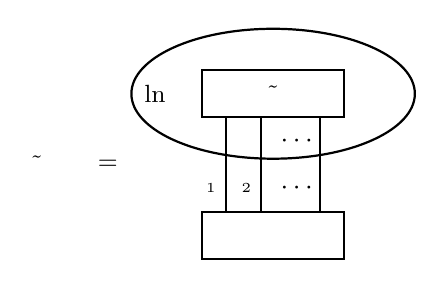
\begin{tikzpicture}[scale=0.3,thick] % , baseline = -3.5pt

\node[anchor=center] (text) at (-8,-5) {\small $\centropyof{\probtensor}{\tilde{\probtensor}}$};

\node[anchor=center] (text) at (-5,-5) {\small ${=}$};

\node[anchor=center] (text) at (-3,-2) {\small $\mathrm{ln}$};
\draw (2,-2) ellipse (6 and 2.75);

\draw (-1,-1) rectangle (5,-3);
\node[anchor=center] (text) at (2,-2) {\small $\tilde{\probtensor}$};
\draw (-1,-7) rectangle (5,-9);
\node[anchor=center] (text) at (2,-8) {\small $\probtensor$};
\draw (0,-5)--(0,-3); 
\draw (0,-5)--(0,-7) node[midway,left] {\tiny $\atomlegindexof{1}$}; 
\draw (1.5,-5)--(1.5,-3); 
\draw (1.5,-5)--(1.5,-7) node[midway,left] {\tiny $\atomlegindexof{2}$}; 
\node[anchor=center] (text) at (3,-4) {$\cdots$};
\draw (4,-5)--(4,-3);
\node[anchor=center] (text) at (3,-6) {$\cdots$};
\draw (4,-5)--(4,-7) node[midway,right] {\tiny $\atomlegindexof{\atomorder}$}; 

%\drawatomcore{3.5}{-8}{$\probtensor$}
%\drawatomindices{3.5}{-12}	
%\draw (5.5,-9)--(5.5,-7) node[midway,right] {\tiny $\atomlegindexof{\exformula}$};

\end{tikzpicture}
%	\end{center}
\end{definition}



% Interpretation of MLE as Cross-Entropy Minimization
Comparing with the negative log likelihood we notice that that loss coincides with the cross-entropy between the empirical distribution $\empdistribution$ and $\probtensor$, i.e.
	\[ \lossof{\probtensor} = \centropyof{\empdistribution}{\probtensor} \, . \]
We can therefore rewrite Problem~\ref{prob:parameterMaxLikelihood} as minimization of cross-entropies and of Kullback Leibler divergences as
\begin{align*}
	\argmin_{\probtensor\in\Gamma} \lossof{\probtensor} 
	= \argmin_{\probtensor\in\Gamma} \centropyof{\empdistribution}{\probtensor} 
	= \argmin_{\probtensor\in\Gamma} \kldivof{\empdistribution}{\probtensor} \, .
\end{align*}
	








\subsection{Forward Mapping in Exponential Families} 

\red{Integrate: Selection encodings suffice for variational methods, relational encodings of statistics are required for markov network instantiations of exponential families.}

Following \cite{wainwright_graphical_2008}, we can characterize the forward mapping as a variational problem.



\subsubsection{Variational Formulation}

Besides the direct computation of the mean parameter tensor we can give a variational characterization of the forward mapping.
This is especially useful, when the contraction is intractable, for example because the tensor $\expdist$ is infeasible to create.

We have
\begin{align*}
	\forwardmap(\canparam)  = \argmax_{\meanparam\in\meanset}  \contractionof{\meanparam,\canparam}{\varnothing} + \sentropyof{\probtensor^{\meanparam}} 
\end{align*}
where 
\begin{align*}
	 \meanset = \{  \contractionof{\probtensor,\sencodingof{\sstat}}{\selvariable}  :  \probtensor \quad \text{a distribution} \}
\end{align*}

% Forward mapping as gradient of A
In \cite{wainwright_graphical_2008}: Forward mapping coincides with gradient, i.e. $\meanparam = \nabla \cumfunction(\canparam)$.


\subsubsection{Mean Field Method}

Restrict the maximum over the mean parameters of efficiently contractable distributions and get a lower bound.

We rewrite 
\begin{align*}
	\max_{\meanparam\in\meanset}  \sbcontractionof{\meanparam, \canparam} + \sentropyof{\probtensor^{\meanparam}} 
	=
	\max_{\probtensor} \sbcontraction{\energytensor, \probtensor} + \sentropyof{\probtensor}
\end{align*}
where
	\[ \energytensor = \sbcontractionof{\sstat,\canparam}{\shortcatvariables} \, . \]

We now restrict the distributions in the maximum.
Typically we use the family of independent distributions, also called naive mean field method.
The naive mean field is the approximation by distributions of independent random variables $\legcoreof{\atomenumerator}$, that is
\begin{align*}
	\argmax_{\legcoreof{\atomenumerator} \, : \, \atomenumeratorin} \contractionof{\{\energytensor\} \cup \{\legcoreof{\atomenumerator} \, : \, \atomenumeratorin\}}{\varnothing}
	+ \sum_{\atomenumeratorin} \sentropyof{\legcoreof{\atomenumerator}} \, . 
\end{align*}

Algorithm~\ref{alg:NMF} is the alternation of legwise updates until a stopping criterion is met.

\begin{algorithm}[h!]
\caption{Naive Mean Field Approximation}\label{alg:NMF}
\begin{algorithmic}
\For{$\atomenumeratorin$}
	\State 
		\[ \legcoreofat{\atomenumerator}{\catvariableof{\atomenumerator}} = \onesat{\catvariableof{\atomenumerator}}  \]
\EndFor
\While{Stopping criterion is not met}
	\For{$\atomenumeratorin$}
		\State 
			\[ \legcoreofat{\atomenumerator}{\catvariableof{\atomenumerator}} 
			= \normationofwrt{ \expof{ \contractionof{ \{\energytensor[\shortcatvariables] \} \cup
				\{\legcoreofat{\secatomenumerator}{\catvariableof{\secatomenumerator}}\} }{\shortcatvariables} }
			}{\catvariableof{\atomenumerator}}{\varnothing} \]
\EndFor
\EndWhile
\end{algorithmic}
\end{algorithm}


%% Structured Variational approximation
More generically, one can use any Markov Network as the approximating family. % Also any exponential family?
Let $\graph$ be any hypergraph, we define the problem
\begin{align}\tag{$\mathrm{P}_{\mnexpfamily, \probtensor}$}\label{prob:structuredApproximation}
	\argmax_{\probtensor\in \mnexpfamily} \contractionof{\{\energytensor, \probtensor\}}{\varnothing} + \sentropyof{\probtensor}
\end{align}

\begin{theorem}
	The Markov Network with hypercores $\{ \hypercoreat{\edge} : \edgein \}$ is a stationary point for Problem~\ref{prob:structuredApproximation}, if for all $\edgein$
	\begin{align*}
	\hypercoreofat{\edge}{\catvariableof{\edge}}
	= \lambda\cdot \expof{
	\frac{
		\contractionof{\{\energytensor\}\cup\{
		\hypercoreat{\secedge} : \secedge\neq\edge
		\}}{\catvariableof{\edge}} 
	}{
		\contractionof{\{
		\hypercoreat{\secedge} : \secedge\neq\edge
		\}}{\catvariableof{\edge}} 
	}
	+ \sum_{\secedge\neq\edge} 
		\frac{
		\contractionof{\{\lnof{\hypercoreat{\secedge}}\}\cup\{
		\hypercoreat{\secedge} : \secedge\neq\edge
		\}}{\catvariableof{\edge}} 
	}{
		\contractionof{\{
		\hypercoreat{\secedge} : \secedge\neq\edge
		\}}{\catvariableof{\edge}} 
	}
	}
	\end{align*}
	for any $\lambda>0$ (e.g. by the norm).
	Here, the quotient denotes the coordinatewise quotient.
\end{theorem}
\begin{proof}
	By first order condition on the objective.
\end{proof}

%% KL Divergence
The mean field method corresponds with minimization of the KL Divergence to the efficiently contractable family, i.e. the I-projection onto the family.

\begin{theorem}
	For any hypergraph $\graph$ and energy tensor $\energytensor$ we have 
	\begin{align*}
		\argmax_{\probtensor\in \mnexpfamily} \contractionof{\{\energytensor, \probtensor\}}{\varnothing} + \sentropyof{\probtensor}
		= \argmax_{\probtensor\in \mnexpfamily} \kldivof{\expdistof{(\graph,\canparam)}}{\normationofwrt{\expof{\energytensor}}{\shortcatvariables}{\varnothing}}
	\end{align*}
	Problem~\ref{prob:structuredApproximation} is thus the I-projection onto the exponential family $\mnexpfamily$.
\end{theorem}
\begin{proof}
%	This follows from the fact, that the objective is the cross-entropy and the position of the maximum is invariant under substracting $\sentropyof{\probtensor}$.
	By rearranging the objective to the KL divergence.
\end{proof}


\subsubsection{Mode Search by annealing}

Finding the mode of a distribution is related to the forward mapping of $\invtemp\cdot\canparam$: $\meanparam$ to a delta distribution (or in the convex hull of multiple maxima) in the limit.

% Annealing effect on the optimization problem
This is because 
\begin{align*}
	\argmax_{\meanparam\in\meanset}  \contractionof{\meanparam,\canparam}{\varnothing} 
\end{align*}
is taken at an extreme point in $\meanset$ (since linear objective over closed convex set), which is a delta distribution of a set and
\begin{align*}
	\argmax_{\meanparam\in\meanset}  \contractionof{\meanparam,\invtemp\cdot\canparam}{\varnothing} + \sentropyof{\probtensor^{\meanparam}} 
	= 
	\argmax_{\meanparam\in\meanset}  \contractionof{\meanparam,\canparam}{\varnothing} + \frac{1}{\invtemp} \cdot \sentropyof{\probtensor^{\meanparam}} 	
\end{align*}
thus the entropy term is neglectible for large $\invtemp$.
A more precise argument is using a limit of the maxima and can be found in Theorem~8.1 in \cite{wainwright_graphical_2008}





\subsection{Backward Mapping in Exponential Families}

We find one backward mapping as the dual problem to the forward mapping.

\subsubsection{Variational Formulation}

The backward mapping to $\datamean = \sbcontractionof{\empdistribution, \sstat}{\selvariable}$ is Maximum Likelihood estimation and the solution of the maximum entropy problem.

\begin{lemma}
	Let there be a sufficient statistic $\sstat$.
	The map $\backwardmap: \rr^{\statorder}\rightarrow \rr^{\statorder}$ defined as
	\begin{align*}
		\backwardmap(\meanparam) = \argmax_{\canparam\in\rr^{\statorder}}  \contractionof{\meanparam,\canparam}{\varnothing} - \cumfunctionof{\canparam} \, . 
	\end{align*}
	is a backward mapping.
\end{lemma}
\begin{proof}
	From duality, see Theorem~3.4 in \cite{wainwright_graphical_2008}.
\end{proof}

% Gradient property
In \cite{wainwright_graphical_2008}: The objective is the conjugate dual $\dualcumfunction$ of $\cumfunction$, and backward mapping has an expression by the gradient, i.e. $\canparam = \nabla \dualcumfunction(\meanparam)$.


\begin{theorem}[Moment Matching Criteria]\label{the:MM}
	We have that $\canparam$ is a solution of the backward problem at $\genmean$, if and only if 
		\[ \sbcontractionof{\expdist,\sstat}{\selvariable} = \genmean[\selvariable] \, . \]
\end{theorem}

The equation in seeTheorem~\ref{the:mm} are called moment matching, since the moment of the empirical distribution is matched by the moment of the fitting distribution.




\subsubsection{Connection with Maximum Likelihood Estimation}

% Backward mapping
Backward mapping coincides with the Maximum Likelihood Estimation as we show next.

% From Parameter Estimation: When taking hypothesis to be exponential family
We now take $\Gamma$ to coincide with an exponential family $\expfamily$ for a sufficient statistic $\sstat$.

% Cross entropy
The objective is the cross entropy between a distribution with $\meanparam$ and the distribution $\expdistof{\sstat,\canparam}$.

\begin{lemma}
	Let $\sstat\in\facspace\otimes\rr^{\statorder}$ be a sufficient statistic and $\gendistribution\in\facspace$ a probability distribution.
	For any member $\expdist\in\expfamily$ we have
		\[ \centropyof{\gendistribution}{\expdist} = \sbcontraction{\canparam,\genmean} - \cumfunctionof{\canparam} \]
	where 
		\[ \genmean = \sbcontractionof{\gendistribution,\sstat}{\catvariableof{\sstat}} \,  \]
	and 
		\[ \cumfunction(\canparam) = \lnof{\contraction{\expof{\expenergy}}} \, . \]
	The M-projection of $\gendistribution$ onto $\expfamily$ is  $\expdistof{(\sstat,\estcanparam)}$ for
		\[ \estcanparam\in \argmax_{\canparam}  \contraction{\canparam, \genmean} - \cumfunctionof{\canparam} \, .  \]
\end{lemma}
\begin{proof}
	By decomposing 
	\begin{align*}
		\expdist 	& = \normationofwrt{\expof{\contractionof{\{\sstat, \canparam\}}{\shortcatvariables}}}{\shortcatvariables}{\varnothing} \\
				& = \frac{\expof{\expenergy}}{\contractionof{\{\expof{\expenergy}\}}{\varnothing}}
	\end{align*}
	we get
	\begin{align*}
		\lnof{\expdist} & = \lnof{\expof{\expenergy}} - \onesat{\shortcatvariables} \cdot \contractionof{\expof{\expenergy}}{\varnothing} \\ 
		& = \expenergy - \cumfunction(\canparam) \cdot \onesat{\shortcatvariables}  \, .
	\end{align*}
	If follows that
	\begin{align*}
		\centropyof{\gendistribution}{\expdist} 
		&=  \sbcontraction{\gendistribution,\lnof{\expdist}} \\
		&=  \sbcontraction{\gendistribution,\expenergy} - \cumfunction(\canparam) \cdot \contractionof{\{\gendistribution\}}{\varnothing}   \\
		&= \sbcontraction{\canparam, \genmean} - \cumfunction(\canparam) \, . 
	\end{align*}
\end{proof}




%\subsection{Maximum Likelihood and Maximum Entropy for Exponential Families}

Parameter Estimation is the M-Projection of a distribution onto the exponential family.

\begin{theorem}[\cite{wainwright_graphical_2008}]\ref{the:parEstToBackwardMap}
	Given any probability distribution $\probof{\shortcatvariables}$ and a exponential family defined by the sufficient statistic $\sstat$, the M-Projection onto the family is the distribution $\probtensorof{(\sstat,\estcanparam)}$ where
	\begin{align*}
		\estcanparam = \backwardmap(\contractionof{\probtensor,\sstat}{\catvariableof{\sstat}}) \, .
	\end{align*}
\end{theorem}
\begin{proof}
	$\contractionof{\probtensor,\sstat}{\catvariableof{\sstat}}$ is in $\imageof{\forwardmap}$ and MLE has a variational characterization with maximum at the dual $\estcanparam$, see \cite{wainwright_graphical_2008}.
\end{proof}





\subsubsection{Connection with Maximum Entropy}\label{sec:maxEntDuality}


%Primal: Maximum likelihood principle.
%\begin{align*}
%	\argmax_{\weight\in\rr^{\cardof{\formulaset}}} \lossof{\formulaset,\weight}
%\end{align*}


The Maximum entropy problem with respect to matching expected statistics is
\begin{align}\tag{$\mathrm{P}_{\sentropyof{}, \genmean}$}\label{prob:maxEntropy}
	\argmax_{\probtensor} \sentropyof{\probtensor} \quad \text{subject to} \quad  \sbcontractionof{\probtensor,\sencodingof{\sstat}}{\selvariableof{\sstat}} =  \genmean
\end{align}
where the optimization is over all probability distributions $\probtensor$.





\begin{theorem}\label{the:maxEntMaxLikeDuality}
	Let $\sstat$ be a map and $\gendistribution$ be any distribution of $\atomstates$ and define
		\[ \genmean = \sbcontractionof{\gendistribution,\sencodingof{\sstat}}{\selvariableof{\sstat}} \, .  \]
	Then the solution of \ref{prob:maxEntropy} coincides with the member $\expdistof{(\sstat,\estcanparam)}$ of the exponential family $\expfamily$ where
		\[ \estcanparam = \backwardmap(\genmean)\]
	for a backward map $\backwardmap$ of $\expfamily$.
\end{theorem}
\begin{proof}
	Classical result based on duality of maximum entropy and maximum likelihood, shown e.g. in Koller Book.
\end{proof}

%
Theorem~\ref{the:maxEntMaxLikeDuality} states, that when the maximum entropy problem has a solution (i.e. $\genmean\in\meanset$), then the solution is in the exponential family to the statistic $\sstat$.



\subsubsection{Alternating Algorithms to Approximate the Backward Map}\label{sec:alternatingBackwardMap}


\red{While the forward map always has a representation in closed form by contraction of the probability tensor, the backward map in general fails to have a closed form representation.
Computation of the Backward map can instead be performed by alternating algorithms.} % Are these fixpoint iterations?


Alternate through the coordinates of the statistics and adjust $\canparamat{\selvariable=\statenumerator}$ to a minimum of the likelihood, i.e. where
\begin{align*}
	0 = \frac{\partial}{\partial \canparamat{\selvariable=\statenumerator}} \lossof{\expdist}
\end{align*}

% Moment matching
This condition is equal to the collection of moment matching equations (see Theorem~\ref{the:mm})
\begin{align*}
	\sbcontractionof{\expdist,\sencodingof{\sstat}}{\selvariable=\statenumerator} = \sbcontraction{\empdistribution,\sencodingof{\sstat}}{\selvariable=\statenumerator} \, . 
\end{align*}


\begin{lemma}\label{lem:mmContractionEquation}
	For any sufficient statistic $\sstat$ a parameter vector $\canparam$ and a $\statenumeratorin$ we define
	\begin{align*}
	 	\hypercoreat{\catvariableof{\sstat_\statenumerator}} 
		= \contractionof{\{\rencodingof{\sstat}\}\cup\{\headcoreof{\tilde{\statenumerator}} : \tilde{\statenumerator} \in [\statorder], \tilde{\statenumerator}\neq\statenumerator\}}{\catvariableof{\sstat_\statenumerator}} \, . 
	\end{align*}
	Then the moment matching condition for $\sstat_\statenumerator$ relative to $\canparam$ and $\meanparam_\sstat$ is satisfied for any $\canparamat{\selvariable=\statenumerator}$ with
	\begin{align*}
		\sbcontraction{\headcoreof{\statenumerator}, \idrestrictedto{\imageof{\sstat_\statenumerator}}, \hypercoreat{\selvariable_\sstat}}
		= \sbcontraction{\headcoreof{\statenumerator}, \hypercoreat{\selvariable_\sstat}} \cdot \meanparam_\statenumerator \, . 
	\end{align*}
\end{lemma}
\begin{proof}
	We have
	\begin{align*}
		\expdist = \frac{
			\contractionof{\{\headcoreof{\statenumerator}, \hypercore \}}{\shortcatvariables}
		}{
			\sbcontraction{\headcoreof{\statenumerator}, \hypercore}
		}
	\end{align*}
	and 
	\begin{align*}
		\contractionof{\{\expdist, \sstat_\statenumerator\}}{\varnothing} 
		= \frac{
			\contractionof{\{\headcoreof{\statenumerator}, \idrestrictedto{\imageof{\sstat_\statenumerator}}, \hypercore \}}{\shortcatvariables}
		}{
			\contractionof{\{\headcoreof{\statenumerator}, \hypercore\}}{\varnothing}
		} \, . 
	\end{align*}
	Here we used
		\[ \sstat_\statenumerator = \contractionof{\{\headcoreof{\statenumerator}, \idrestrictedto{\imageof{\sstat_\statenumerator}}\}}{\shortcatvariables} \]
	and redundancies of copies of relational encodings.
	It follows that 
	\begin{align*}
		\contractionof{\{\expdist,\sstat_\statenumerator\}}{\varnothing} = \contractionof{\{\empdistribution,\sstat_\statenumerator\}}{\varnothing}
	\end{align*}
	is equal to
	\begin{align*}
		\contractionof{\{\headcoreof{\statenumerator}, \idrestrictedto{\imageof{\sstat_\statenumerator}}, \hypercoreat{\selvariable_\sstat}  \}}{\varnothing}
		= \contractionof{\{\headcoreof{\statenumerator}, \hypercoreat{\selvariable_\sstat}  \}}{\varnothing} \cdot \meanparam_\statenumerator \, . 
	\end{align*}	
\end{proof}

% Alternation necessary
The steps have to be alternated until sufficient convergence, since matching the moment to $\statenumerator$ by modifying $\canparamat{\selvariable=\statenumerator}$ will in general change other moments, which will have to be refit.


%Coordinate descent
An alternating optimization is the coordinate descent of the negative likelihood, seen as a function of the coordinates of $\canparam$, see Algorithm~\ref{alg:AMM}.
Since the log likelihood is concave, the algorithm converges to a global minimum.





\begin{algorithm}[h!]
\caption{Alternating Moment Matching}\label{alg:AMM}
\begin{algorithmic}
\State Set $\canparamat{\selvariable}=0$
\State Compute $\datameanat{\selvariable}= \sbcontractionof{\empdistribution,\sencodingof{\sstat}}{\selvariable}$
%\For{$\statenumeratorin$}
%	\State Set $\canparamat{\selvariable=\statenumerator}=0$ 
%	\State Compute $\meanparam_\statenumerator^{\datamap} = \contractionof{\{\empdistribution,\sstat_\statenumerator\}}{\varnothing} $ % Or give those as input!
%\EndFor
\While{Stopping criterion is not met}
\For{$\statenumeratorin$}
	\State Compute 
		\begin{align*}
			\hypercoreofat{\statenumerator}{\catvariableof{\sstat_\statenumerator}} 
			= \contractionof{\{\rencodingof{\sstat}\}\cup\{\headcoreof{\tilde{\statenumerator}} : \tilde{\statenumerator} \in [\statorder], \tilde{\statenumerator}\neq\statenumerator\}}{\catvariableof{\sstat_\statenumerator}} 
		\end{align*}
	\State Set $\canparamat{\selvariable=\statenumerator}$ to a solution of 
	\begin{align*}
		\contraction{\{\headcoreof{\statenumerator}, \idrestrictedto{\imageof{\sstat_\statenumerator}}, \hypercoreof{\statenumerator} \}}
		= \contraction{\{\headcoreof{\statenumerator},\hypercoreof{\statenumerator} \}} \cdot \meanparam_\statenumerator^{\datamap} \, . 
	\end{align*}
\EndFor
\EndWhile
\end{algorithmic}
\end{algorithm}


% 
In general, if $\imageof{\sstat_\statenumerator}$ contains more than two elements, there exists no closed form solutions.
We will investigate the case of binary images, where there are closed form expressions, later in Section~\ref{sec:alternatingParEstMLN}.


%
The computation of $\hypercore_\statenumerator$ in Algorithm~\ref{alg:AMM} can be intractable and be replaced by an approximative procedure based on message passing schemes.


